% This file was created by matlab2tikz.
%
\definecolor{mycolor1}{rgb}{0.00000,0.44700,0.74100}%
%
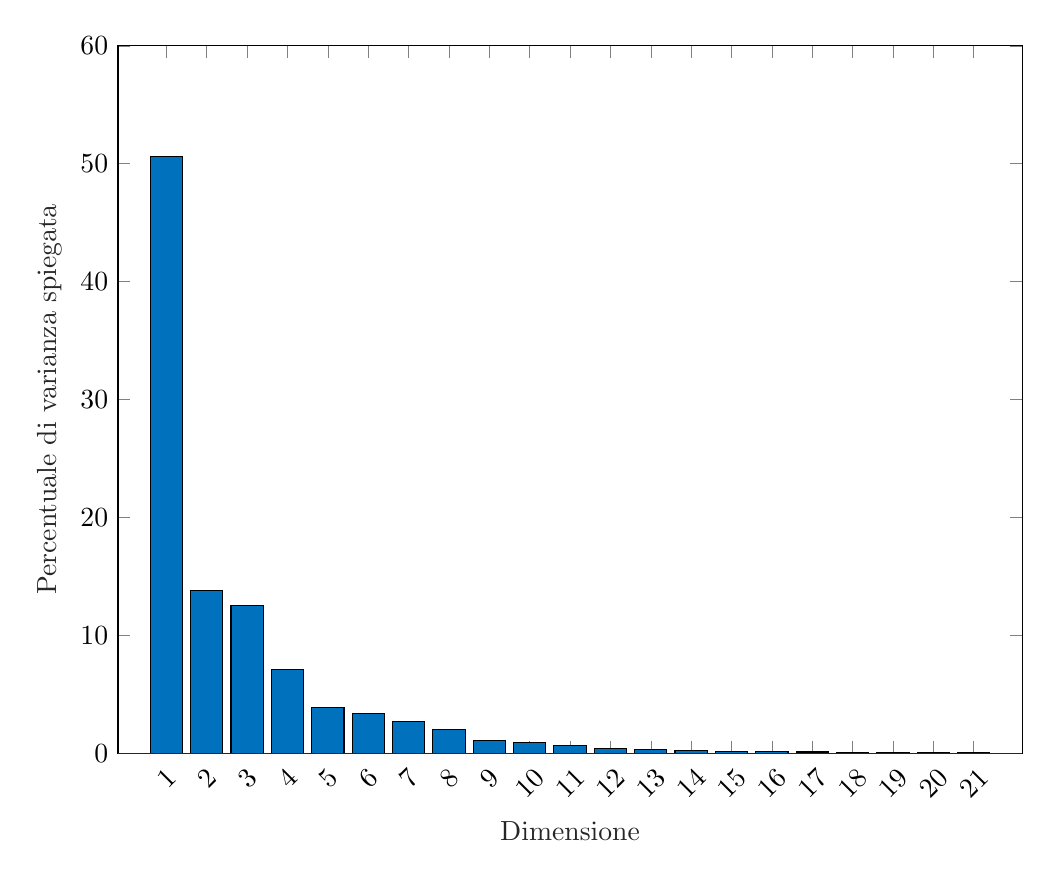
\begin{tikzpicture}

\begin{axis}[%
width=4.521in,
height=3.537in,
at={(0.758in,0.509in)},
scale only axis,
bar shift auto,
xmin=-0.2,
xmax=22.2,
xtick={ 1,  2,  3,  4,  5,  6,  7,  8,  9, 10, 11, 12, 13, 14, 15, 16, 17, 18, 19, 20, 21},
xticklabel style={rotate=45},
xlabel style={font=\color{white!15!black}},
xlabel={Dimensione},
ymin=0,
ymax=60,
ylabel style={font=\color{white!15!black}},
ylabel={Percentuale di varianza spiegata},
axis background/.style={fill=white}
]
\addplot[ybar, bar width=0.8, fill=mycolor1, draw=black, area legend] table[row sep=crcr] {%
1	50.5858591666905\\
2	13.8045026896465\\
3	12.5552629319904\\
4	7.09897984468841\\
5	3.8506062851651\\
6	3.34426315079743\\
7	2.66974822615883\\
8	1.97748126185028\\
9	1.04416562734188\\
10	0.882132103168467\\
11	0.649054535879739\\
12	0.400507145860743\\
13	0.328297787193329\\
14	0.220070868341111\\
15	0.169516685172436\\
16	0.14015154641536\\
17	0.0991393489304061\\
18	0.0622273867356755\\
19	0.0375917262088089\\
20	0.0304749102737549\\
21	0.0201945158185743\\
};
\addplot[forget plot, color=white!15!black] table[row sep=crcr] {%
-0.2	0\\
22.2	0\\
};
\end{axis}
\end{tikzpicture}%